\graphicspath{./Images}
\section{Introduction}
In the automotive industry, the passive crash structures of a vehicle is tested by standardized testing procedures for the homologation of the vehicles. These testing procedures often involve the use of a low-cost representation of the passive crash structure of another vehicle to act as a collision partner for the vehicle that is under assessment. This collision partner is often referred to as a Mobile Progressive Deformable Barrier (MPDB). Such an MPDB consists of a trolley with an energy absorbing barrier attached to the front. In Figure \ref{Ch1_MDBtoV_cut} an example of a car-to-MPDB test is illustrated. Different test set-ups are used for the assessment of a vehicle, with variations in for example approach angles, approach velocities and barrier types. 
\begin{figure}[H]
    \centering
    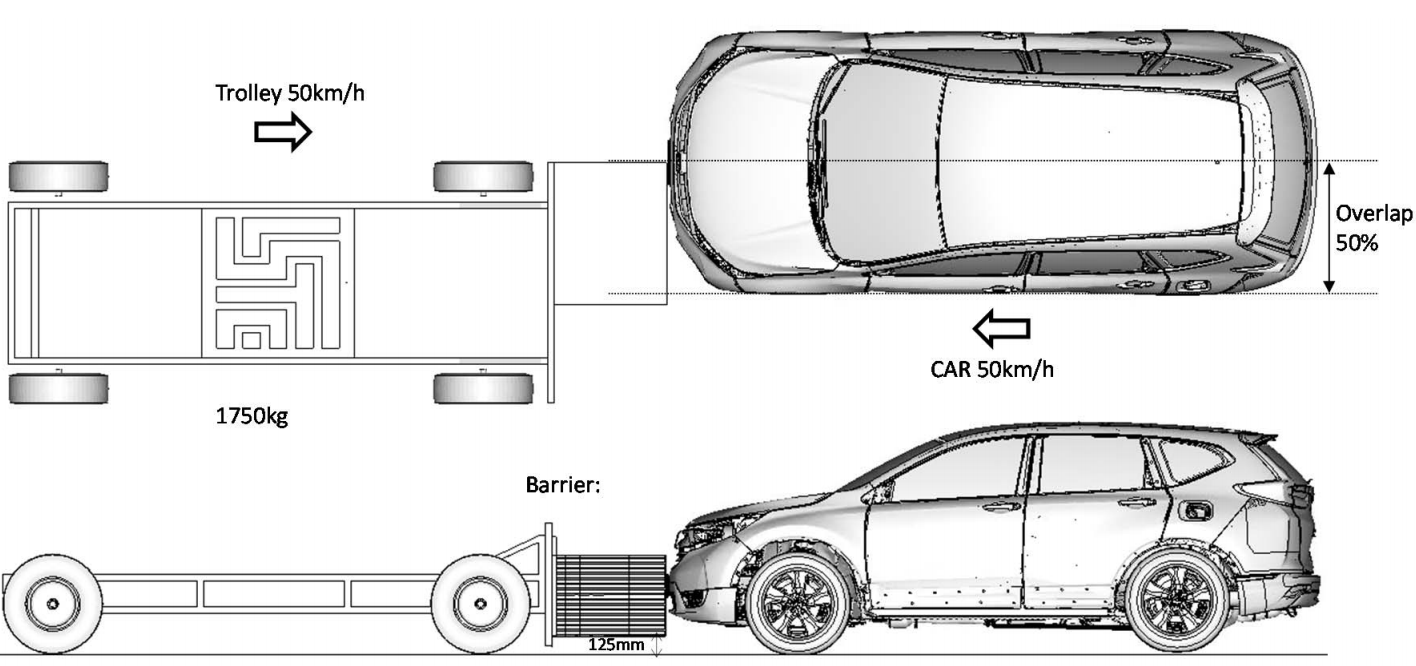
\includegraphics[width=0.8\linewidth]{./Images/Ch1/Ch1_MDBtoV_cutv2.PNG}
    \caption{Oblique car-to-MPDB test for a small SUV. \cite{MDBtoV}}
    \label{Ch1_MDBtoV_cut}
\end{figure}

\noindent Since performing these full scale crash tests is expensive and time-consuming, extensive numerical simulations are performed during the development phase of a vehicle. In order to perform those simulations, both the passive crash structure of the vehicle itself as well as the deformable crash barrier must be modeled accurately. \\
\newline
As was mentioned, different types of energy absorbing barriers are used for different test set-ups. An example of a barrier is depicted in Figure \ref{Ch1_honeycombphoto1}. The barriers are typically composed of multiple segments of aluminium honeycomb material (grey) enclosed by aluminium cladding sheets (blue). Figure \ref{Ch1_honeycombphoto2} shows the cell geometry of the aluminum honeycomb material.

\begin{figure}[H]
    \centering
    \begin{subfigure}[b]{0.54\textwidth}
    \centering
        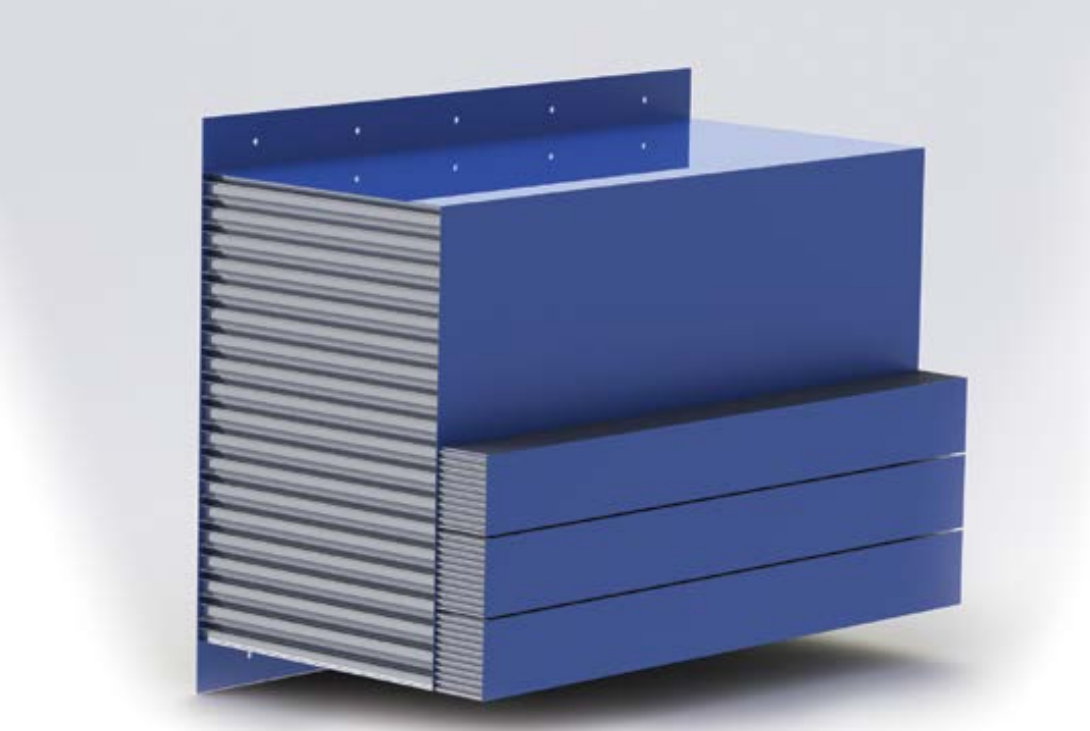
\includegraphics[width=0.98\textwidth]{./Images/Ch1/Ch1_wg11.PNG}
        \caption{WG11 deformable barrier. \cite{plascore}}
        \label{Ch1_honeycombphoto1}
    \end{subfigure}
    \quad
    \begin{subfigure}[b]{0.32\textwidth}
        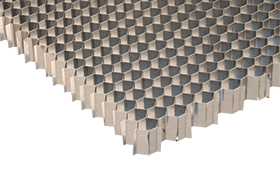
\includegraphics[width=0.98\textwidth]{./Images/Ch1/Ch1_honeycombphoto.jpg}
        \caption{Honeycomb cell structure. \cite{plascore}}
        \label{Ch1_honeycombphoto2}
    \end{subfigure}
    \caption{}
    \label{Ch1_honeycombphoto}
\end{figure}
Due to the geometry of the material, the mechanical behaviour of the aluminium honeycomb is complex. The macroscopic response is governed by micro- and meso-scale phenomena such as plastic buckling, cell rupture and debonding \cite{popp}.\\
A significant amount of research has been invested in the modeling of this type of material behavior. Roughly two types of modeling approaches can be distinguished, based on the type of element that is used for describing the material behavior: shell elements or continuum elements, visualized in Figure \ref{Ch2_shellsolid}. \\
\begin{figure}[H]
    \centering
    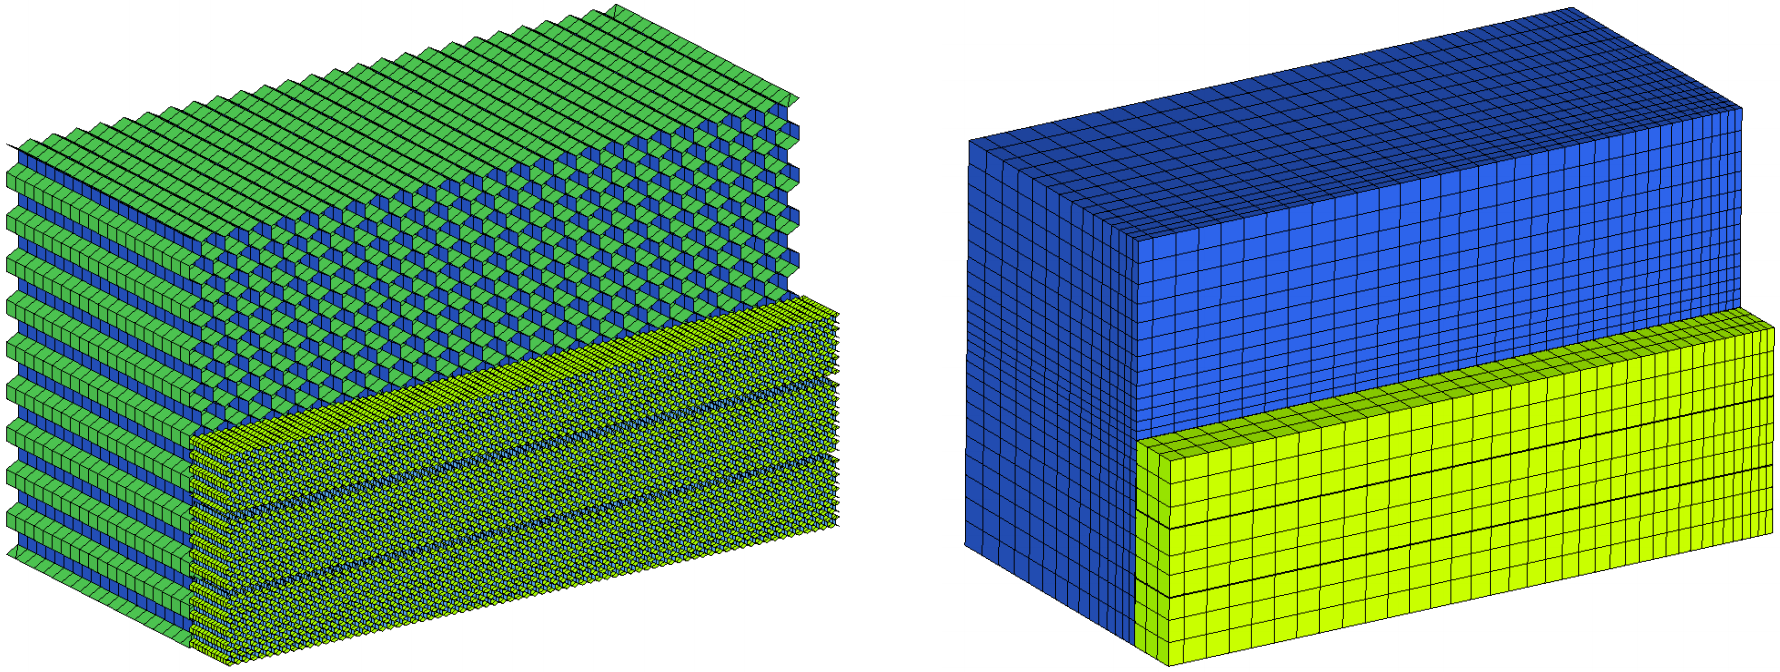
\includegraphics[width=0.8\linewidth]{./Images/Ch1/Ch1_niedermeyer_shellsolid.PNG}
    \caption{Shell element model (left) and continuum element model (right). \cite{niedermeyer}}
    \label{Ch2_shellsolid}
\end{figure}
Since the hexegonal cell structure of the material is captured in the shell models, this type of models inherently capture the geometric effects of the material. The continuum models appear simpler at first glance. However, the geometric effects are not inherently captured and must be accounted for by the material model.\\

{\color{red}{MEER TYPEN}}

\subsection{Goal and outline}
Therefore, the goal of this work is to {\color{red}{INSERT GOAL}}. In order to achieve this goal, the continuum model of Van Iersel are discussed in Section 2. In Section 3, a finite deformation model is proposed to eliminate the undesired effects in the continuum model of Van Iersel. {\color{red}{Section 4....}}.